%%%%%%%%%%%%%%%%%%%%%%%%%%%%%%%%%%%%%%%%%
% Tutorial
% LaTeX Template
% Version 1.0 (09/27/17)
%
% Author:
% Ben Roose (ben.roose@wichita.edu)
%
% Original template author:
% Adam Glesser (adamglesser@gmail.com)
% www.LaTeXTemplates.com
%
% License:
% CC BY-NC-SA 3.0 (http://creativecommons.org/licenses/by-nc-sa/3.0/)
%
%%%%%%%%%%%%%%%%%%%%%%%%%%%%%%%%%%%%%%%%%

\documentclass[12pt]{article}

\usepackage{graphicx} % Allow import of images
\usepackage{subcaption} % Required for side-by-side sub figures
\graphicspath{ {images/} } % Relative path to images directory
\usepackage[margin=1in]{geometry} % Required to make the margins smaller to fit more content on each page
\usepackage[linkcolor=blue]{hyperref} % Required to create hyperlinks to questions from elsewhere in the document
\hypersetup{pdfborder={0 0 0}, colorlinks=true, urlcolor=blue} % Specify a color for hyperlinks
\usepackage{todonotes} % Required for the boxes that questions appear in
\usepackage{tocloft} % Required to give customize the table of contents to display questions
\usepackage{microtype} % Slightly tweak font spacing for aesthetics
\usepackage{palatino} % Use the Palatino font

\setlength\parindent{0pt} % Removes all indentation from paragraphs

% Create and define the list of questions
\newlistof{questions}{faq}{\large FAQ for SSH access into cslab Linux environment}
% This creates a new table of contents-like environment that will output a file with extension .faq
\setlength\cftbeforefaqtitleskip{3em} % Adjusts the vertical space between the title and subtitle
\setlength\cftafterfaqtitleskip{1em} % Adjusts the vertical space between the subtitle and the first question
\setlength\cftparskip{.3em} % Adjusts the vertical space between questions in the list of questions

% Create the command used for questions
\newcommand{\question}[1] % This is what you will use to create a new question
{
\refstepcounter{questions} % Increases the questions counter, this can be referenced anywhere with \thequestions
%\hfill
\goodbreak
\par\noindent % Creates a new unindented paragraph
\phantomsection % Needed for hyperref compatibility with the \addcontensline command
\addcontentsline{faq}{questions}{#1} % Adds the question to the list of questions
\todo[inline, color=green!40]{\textbf{#1}} % Uses the todonotes package to create a fancy box to put the question
%\vspace{0.5em} % White space after the question before the start of the answer
}

% Uncomment the line below to get rid of the trailing dots in the table of contents
%\renewcommand{\cftdot}{}

% Uncomment the two lines below to get rid of the numbers in the table of contents
%\let\Contentsline\contentsline
%\renewcommand\contentsline[3]{\Contentsline{#1}{#2}{}}

\begin{document}

%----------------------------------------------------------------------------------------
%	TITLE AND LIST OF QUESTIONS
%----------------------------------------------------------------------------------------

\begin{center}
\Huge{\bf \emph{EECS Tutorial: cslab Linux Environment SSH Access}} % Main title
\end{center}

\listofquestions % This prints the subtitle and a list of all of your questions
\bigskip % Create a gap between list and first question

\newpage % Comment this if you would like your questions and answers to start immediately after table of questions

%----------------------------------------------------------------------------------------
%	QUESTIONS AND ANSWERS
%----------------------------------------------------------------------------------------
\begin{flushleft}

\question{General Information regarding accessing cslab Linux environment using SSH}\label{ssh_client_linux}
\begin{itemize}
  \item \textbf{Please only connect into the cslab environment with an SSH client if you have previous experience in using SSH and the Linux command-line. If you are new to Linux, please use the cslab \textit{Guacamole} web-browser interface.}
  \item SSH uses network port 22. If you are accessing cslab via SSH on WSU campus, ensure you are connected wirelessly to ``WSU Secure'' or using an Ethernet connected computer. ``WSU Guest'' wireless prohibits port 22 connections and your SSH session will fail to connect.
  \item You can only access cslab using SSH public key authentication. You cannot access cslab over SSH using your myWSU password.
  \item The cslab-nodes are located inside a virtual private network. These internal nodes are only SSH accessible via the \texttt{cslab-bastion.cs.wichita.edu} jumphost. Any external connection into the cslab environment must proxy connect through the \texttt{cslab-bastion}.
  \item \texttt{cslab-bastion.cs.wichita.edu} and \texttt{cslab-sftp.cs.wichita.edu} can be used as SCP or SFTP file-server hosts with SSH clients, such as \textit{OpenSSH}, or graphical SFTP clients, such as \textit{Filezilla}.
  \item This tutorial will help you configure your SSH client to make a proxy connection into cslab via \texttt{cslab-bastion} and to set up SSH public key authentication.
  \item \textbf{ONLY USE THE CSLAB-BASTION AS A PROXY/JUMPHOST INTO THE CSLAB-NODES OR AS AN SCP/SFTP SERVER. DO NOT DIRECTLY SSH INTO THE CSLAB-BASTION FOR OTHER TASKS!}
\end{itemize}

%% \question{How do I access cslab Linux environment via \textit{PuTTY} on Microsoft Windows?}\label{ssh_client_windows}
  
%% \subsection*{Using \textit{PuTTY} SSH client on Microsoft Windows:}
%% \begin{enumerate}
%% %% \item You can download pre-configured \textit{PuTTY} session and host key configurations for importing into your Windows registry from this link.

%%   \item Download the full \textit{PuTTY} package from \href{https://www.chiark.greenend.org.uk/~sgtatham/putty/latest.html}{Simon Tatham's official download webpage} and install all \textit{PuTTY} utilities. You cannot connect to cslab with just the \textit{PuTTY} client.
%%   \item Run the 

%%   \item Open \textit{PuTTY} and in [Session] category add a new SSH connection with \break [Host Name] as \texttt{cslab-bastion.cs.wichita.edu} and [Port] as \texttt{22}.

%%   \item In [Connection--Data] category add your myWSU\_ID into [Auto-login username].
%%   \item In [Connection--SSH] category add the text \texttt{ssh cslab} into [Remote command].
%%   \item In [Session] category add a name for the configuration, such as ``cslab environment'' and click \textit{Save}. Saving as ``Default Settings'' will always open with this configuration.

%% \begin{figure}[bh!]
%% \centering
%% \begin{subfigure}{.5\textwidth}
%%   \centering
%%   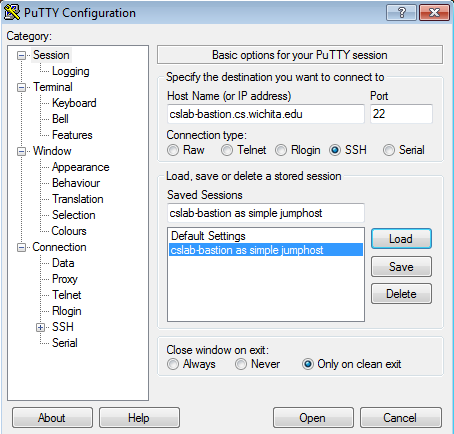
\includegraphics[width=.9\linewidth]{putty_cslab_bastion_session}
%%   %% \caption{A subfigure}
%%   \label{fig:sub1}
%% \end{subfigure}
%% \begin{subfigure}{.5\textwidth}
%%   \centering
%%   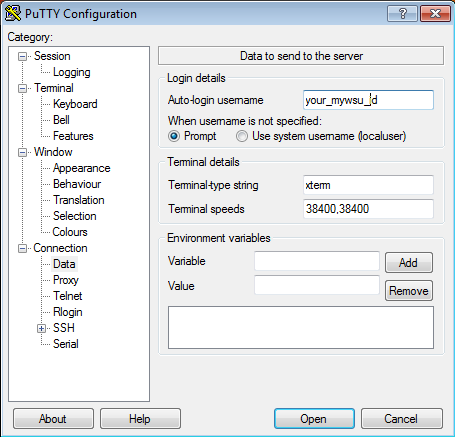
\includegraphics[width=.9\linewidth]{putty_cslab_auto_login_username}
%%   %% \caption{A subfigure}
%%   \label{fig:sub2}
%% \end{subfigure}%
%% \begin{subfigure}{.5\textwidth}
%%   \centering
%%   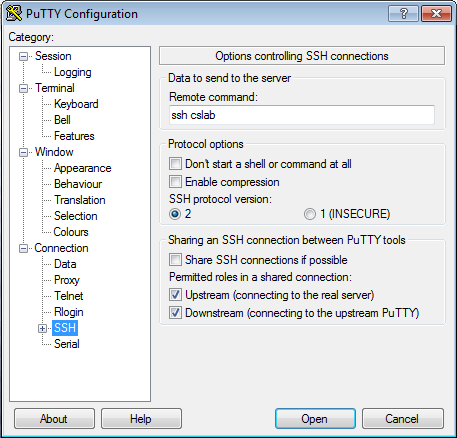
\includegraphics[width=.9\linewidth]{putty_cslab_ssh_remote_command}
%%   %% \caption{A subfigure}
%%   \label{fig:sub3}
%% \end{subfigure}%
%% \caption{\textit{PuTTY} configuration for cslab}
%% \label{fig:putty_config}
%% \end{figure}

%% \goodbreak
%% \item The first time you connect to the cslab environment using SSH, you will be asked to confirm the authenticity of each SSH remote host.
%% \item Ensure the cslab-bastion and cslab host key fingerprints match one of the following SHA256 or MD5 hashes before clicking \textit{Yes}:
%% \begin{verbatim}
%% ECDSA key fingerprint is
%% SHA256:X6dBKj4sqYYPWol6MXSQvGhpIQ6qBxh7mBQhnSw8n64
%% MD5:d8:ba:c6:1c:86:fa:7f:f6:92:4f:c1:02:30:ce:ab:99

%% ED25519 key fingerprint is
%% SHA256:zzozIV7cP1T9C77PLRaevzdzCu21k44lbjd8jaJKS8Q
%% MD5:6d:3d:8e:3a:db:f6:de:33:af:77:01:40:f3:71:1d:14

%% RSA key fingerprint is
%% SHA256:0CUyGZAYMdOd8vTOK3AtM2XTX3lMaGA2NP73rR7s6Ns
%% MD5:75:5a:16:53:1a:7c:c2:4b:99:66:2d:e3:1e:76:f9:c9

%% DSA key fingerprint is
%% SHA256:7zW122xr+aoBb5yiRI96nvdx8Ml07qLKHYwG2Wu6jIM
%% MD5:27:59:53:18:5a:67:71:f6:32:f1:e1:15:e9:e5:fe:b1
%% \end{verbatim}

%% \item You will be prompted twice to enter your myWSU password, once for the cslab-bastion (SSH jumphost/proxy) and once for the internal cslab-node.
%% \item You may see a \texttt{Could not chdir to home directory....} warning. Do not be concerned, this is not a critical error.
%% \item If the SSH connection completed successfully, then you will be presented with a standard shell prompt:

%% \texttt{your\_mywsu\_id@cslab-node-\#:$\sim$\$}
%% \end{enumerate}

%% \question{How do I access the last accessed cslab-node via an SSH client?}\label{ssh -last}

%% \begin{itemize}
%% \item When connecting to the cslab Linux environment using an SSH client, the ballast load-balancer on cslab-bastion will redirect you to one of the available and least used cslab-nodes at time of connection. Since load-balancing is calculated by ballast on a one minute cycle, you may not be redirected to the same cslab-node the next time you connect into cslab using SSH.

%% \item \textbf{Use the following instructions to connect to the last used cslab-node only if/when you need access into a previously running SSH connection. For normal use, your best option is always to connect via \texttt{ssh cslab} and let the ballast load-balancer automatically connect to an available node.}
%% \end{itemize}

%% \subsection*{Using \textit{PuTTY} SSH client on Microsoft Windows:}
%% \begin{enumerate}
%% \item Open \textit{PuTTY} and load the previously created ``cslab environment'' session.
%% \item Change [Connections--Data] configuration category [Remote command] entry to \texttt{ssh cslab-last}.
%% \item \textit{Save} changed configuration as a new [Session] with a different name, such as ``cslab environment last used node''.
%% \item If you need to connect to the last cslab-node you previously accessed using SSH, connect using this newly created \textit{PuTTY} session.
%% \end{enumerate}

%------------------------------------------------
\newpage
\question{How do I access cslab Linux environment via \textit{OpenSSH} on Linux or Mac?}\label{ssh_client_linux}

\subsection*{Configuring the \textit{OpenSSH} client for cslab access:}
\begin{enumerate}
  \item On your Linux or Mac desktop/laptop computer, copy the following host entry into your local user \texttt{$\sim$/.ssh/config} file:
\end{enumerate}

\begin{verbatim}
Host cslab cslab-last cslab.cs.wichita.edu cslab-last.cs.wichita.edu
  ProxyCommand ssh your_mywsu_id@cslab-bastion.cs.wichita.edu ballast %h
  User your_mywsu_id
  IdentityFile ~/.ssh/cslab_rsa
  HostKeyAlias cslab.cs.wichita.edu

Host cslab-sftp cslab-sftp.cs.wichita.edu
  HostName cslab-sftp.cs.wichita.edu
  User your_mywsu_id
  IdentityFile ~/.ssh/cslab_rsa
  HostKeyAlias cslab.cs.wichita.edu
\end{verbatim}
(Note: replace ``your\_mywsu\_id'' with your own 8 character ID number in both \texttt{ProxyCommand} and \texttt{User} lines.)

\begin{enumerate}
  \setcounter{enumi}{1}
  \item Open a command-line terminal emulator window and generate a new SSH public/private key pair for your local user by typing \break
  \texttt{ssh-keygen -t rsa -b 4096 -f $\sim$/.ssh/cslab\_rsa}

  \item Follow the prompts in the command-line as your new SSH key is generated and enter a passphrase you will remember! \break
  \textbf{It is highly recommended to use a passphrase for your SSH key to keep your Linux user account secure.}
  
  \item Open the newly generated SSH public key by typing \break
  \texttt{less $\sim$/.ssh/cslab\_rsa.pub}
  \item Select all the text displayed within \textit{less}, starting with \texttt{ssh-rsa} and ending with the hostname of your local computer.
  \item Copy the text either by right-clicking on the terminal emulator window and selecting copy or by pressing the key combination \textbf{Ctrl+Shift+C}.
  \item Open a web-browser application and follow the \textit{eecs\_tutorial\_cslab\_web\_access} to access \href{https://cslab-gateway.cs.wichita.edu/}{cslab-gateway.cs.wichita.edu}
  \item Once logged into \textit{guacamole}, open a [cslab\_SSH\_CLI\_terminal] connection.
  \item Within the cslab SSH terminal session in your browser, open the \textit{Guacamole} menu sidebar by pressing the key combination \textbf{Ctrl+Alt+Shift}.
  \item Paste the copied text to the remote \textit{Guacamole} [Clipboard] field using your preferred method, i.e. \textbf{Ctrl+V}.
  \item Close the \textit{Guacamole} menu sidebar by pressing the key combination \textbf{Ctrl+Alt+Shift}.
  \item Within the cslab SSH terminal session, open your \texttt{authorized\_keys} file by typing \break
  \texttt{nano $\sim$/.ssh/authorized\_keys}
  \item Paste your locally copied SSH public key into the terminal session by right-clicking on the browser window with your mouse or by pressing the key combination \textbf{Ctrl+Shift+V}.
  \item Ensure you have a blank line at end of the text file by pressing \textbf{Enter} after the text.
  \item Quit \textit{nano} by pressing \textbf{CTRL+X} and follow the prompts at the bottom of the screen to ensure you save the \texttt{authorized\_keys} file.
  \item Ensure correct permissions are set on the \texttt{authorized\_keys} file by typing \break
  \texttt{chmod 600 $\sim$/.ssh/authorized\_keys}
  \item You have now configured your local Linux or Mac computer to directly access cslab via \textit{OpenSSH}. Make sure to properly disconnect and log out of the cslab \textit{guacamole} web-interface once you are done.
  \item \textbf{If you wish to set up more than one local computer with different SSH public/private key pairs for accessing cslab, then you can append additional SSH public keys in your cslab user \texttt{authorized\_keys} file. Make sure to remove no longer used SSH public keys from this file.}
\end{enumerate}

\newpage
\subsection*{Logging into cslab using the \textit{OpenSSH} client:}
\begin{enumerate}
  \item Ensure you have first followed the directions in the previous section to configure your \textit{OpenSSH} client.
  \item In your local computer open a command-line terminal emulator window and connect to the cslab Linux environment by typing \break
  \texttt{ssh cslab}

  \item The first time you connect to the cslab environment using SSH, you will be asked to confirm the authenticity of each SSH remote host, i.e.
\begin{verbatim}
The authenticity of host 'cslab.cs.wichita.edu' can't be established.
ECDSA key fingerprint is [SHA256 or MD5 hash value].
Are you sure you want to continue connecting (yes/no)?
\end{verbatim}

%\break
  \item Ensure the cslab-bastion and cslab host key fingerprints match one of the following SHA256 or MD5 hashes before typing \texttt{yes}:
\begin{verbatim}
ECDSA key fingerprint is
SHA256:X6dBKj4sqYYPWol6MXSQvGhpIQ6qBxh7mBQhnSw8n64
MD5:d8:ba:c6:1c:86:fa:7f:f6:92:4f:c1:02:30:ce:ab:99

ed25519 key fingerprint is
SHA256:zzozIV7cP1T9C77PLRaevzdzCu21k44lbjd8jaJKS8Q
MD5:6d:3d:8e:3a:db:f6:de:33:af:77:01:40:f3:71:1d:14

RSA key fingerprint is
SHA256:0CUyGZAYMdOd8vTOK3AtM2XTX3lMaGA2NP73rR7s6Ns
MD5:75:5a:16:53:1a:7c:c2:4b:99:66:2d:e3:1e:76:f9:c9

DSA key fingerprint is
SHA256:7zW122xr+aoBb5yiRI96nvdx8Ml07qLKHYwG2Wu6jIM
MD5:27:59:53:18:5a:67:71:f6:32:f1:e1:15:e9:e5:fe:b1
\end{verbatim}

  \item When prompted, enter your previously created passphrase to unlock your SSH private key and authenticate into cslab.
  \item If the SSH connection completed successfully, then you will be presented with a standard shell prompt within a cslab node:\break
\texttt{your\_mywsu\_id@cslab-node-\#:$\sim$\$}
\end{enumerate}
\newpage
\subsection*{Logging into your last used cslab-node-\# using the \textit{OpenSSH} client:}
\begin{itemize}
  \item When connecting to the cslab Linux environment using an SSH client, the ballast load-balancer will redirect you to one of the available and least used cslab-nodes at time of connection. Since load-balancing is calculated by ballast on a one minute cycle, you may not be redirected to the same cslab-node the next time you connect into cslab.

  \item \textbf{Use the following instructions to connect to the last used cslab-node only if you need access into a previously running SSH session. For normal use, your best option is always to connect via \texttt{ssh cslab} and let the ballast load-balancer automatically connect you to an available node.}
  \item To connect to the last node you previously accessed using SSH type \break
  \texttt{ssh cslab-last}
\end{itemize}

\subsection*{Running graphical (GUI) applications using the \textit{OpenSSH} client:}
\begin{itemize}
  \item SSH allows for graphical applications to run on a local computer from the remote cslab Linux environment using X11 forwarding.
  \item If you are using Mac OSX, then you may need to install the XQuartz software before using X11 forwarding. Download \href{https://www.xquartz.org}{XQuartz for Mac} and install the software package.
  \item To use X11 forwarding on a per session basis append the \texttt{-X} option flag to your SSH command: \break
  \texttt{ssh -X cslab}
  \item To always use X11 forwarding for connections into cslab, instead of using the \texttt{-X} option flag, add the following line to the \texttt{Host cslab cslab-last ...} entry in your local user \texttt{ $\sim$/.ssh/config} file:
  \begin{verbatim}
  ForwardX11 yes
  \end{verbatim}
\end{itemize} 

%------------------------------------------------

%% \question{How do I copy files from/to the cslab Linux environment via an SSH client?}\label{scp_copying}

\subsection*{Copying files to/from cslab via SCP:}
\begin{itemize}
\item To copy a file from your local computer to your user home directory on cslab using Secure Copy (SCP), type \break
\texttt{scp local\_filename\_or\_path cslab-sftp:$\sim$}

\item To copy a file from your user home directory on cslab to a local directory on your local computer, type \break
\texttt{scp cslab-sftp:$\sim$/remote\_filename\_or\_path local\_directory}
\end{itemize}

%------------------------------------------------

\end{flushleft}
\end{document}
